\part{Testing}\mypartpage
%%%%%%%%%%%%%%%%%%%%%%%%%%%%%%%%%%%%%%%%%%%%%%%%%%%%%%%%%%%%%%%%%%%%%%%%%% 
\begin{frame}{Back on Proofs}
  \begin{block}{Most of you don't see the point of proofs. I know}
    \begin{itemize}
    \item I even agree (to a given point: we need 2 legs to code -- theory and practice)
      \begin{boitequote}{}
        Beware of bugs in the above code; I have only proved it correct, not
        tried it.\hfill -- \emph{D.E. Knuth.}
      \end{boitequote}

    \item \structure{Cost/gain ratio}: if you cannot afford to loose, prove it correct\\
      {\small I hope that Nuclear Power Plants are [partially] proved}
    \item Can give you a competitive advantage:\\
      With these, you may accept more complicated contracts
    \item You're studying in Nancy, there is a local history of algorithm proofs
    \item There will be 1/4 of points on proofs at the exam \ldots
    \end{itemize}
  \end{block}

  \begin{block}{What's expected at the exam}
    \begin{itemize}
    \item Well, that's similar to when you write code
    \item I don't bother a missing \} in the code, as long as the idea is here
    \item I don't bother a partially wrong proof, as long as the method is here
    \end{itemize}
  \end{block}

  \concept{And now, let's see that tests that you guys prefer are even worst}
\end{frame}
%%%%%%%%%%%%%%%%%%%%%%%%%%%%%%%%%%%%%%%%%%%%%%%%%%%%%%%%%%%%%%%%%%%%%%%%%% 
\section{Introduction}
%%%%%%%%%%%%%%%%%%%%%%%%%%%%%%%%%%%%%%%%%%%%%%%%%%%%%%%%%%%%%%%%%%%%%%%%%% 
\begin{frame}[squeeze]{Introduction}
  \begin{block}{Bugs}
    \begin{itemize}
    \item Bugs are inevitable in complex software system
    \item A bug can be very visible or can hide in your code until a much later
      date
    \end{itemize}
  \end{block}\vspace{-.6\baselineskip}
  
  \begin{block}{Bugs can hide very well}
    \begin{description}
    \item[Aug 2009] \alert{8 years} old bug found in Linux 
      {\small(handling not implemented kernel fctions)}\\
      {\footnotesize\url{http://www.theregister.co.uk/2009/08/14/critical_linux_bug/}}
    \item<2->[Jan 2010] Microsoft fixes a \alert{17 years} old bug 
      {\small(in code allowing NT to run 16bits apps)}\\
      {\footnotesize\url{http://www.esecurityplanet.com/features/article.phpr/3860131/Microsoft-Warns-About-17-year-old-Windows-Bug.htm}}
    \item<3->[July 2008] \alert{25 years} old bug found in BSD 
      {\small(\texttt{seekdir()} wrongly implemented)}\\
      {\scriptsize\url{http://www.vnode.ch/fixing_seekdir}}
    \item<4->[July 2008] \alert{33 years} old bug found in Unix 
      {\small(buffer overflow in YACC)}\\
      {\scriptsize\url{http://www.computerworld.com/s/article/9108978/Developer_fixes_33_year_old_Unix_bug}}
    \end{description}
  \end{block}\vspace{-.6\baselineskip}

  \begin{block}<5->{Chasing bugs}
    \begin{itemize}
    \item Once identified, use print statements of IDE's debugger to hunt them
      down
    \item But how to discover all bugs in the system, even those with low
      visibility?
    \item[$\Rightarrow$]<6-> \alert{Testing} and Quality Assurance practices
    \end{itemize}
  \end{block}
\end{frame}
%%%%%%%%%%%%%%%%%%%%%%%%%%%%%%%%%%%%%%%%%%%%%%%%%%%%%%%%%%%%%%%%%%%%%%%%%%
\begin{frame}{Why to test?}
  \begin{boitequote}{E. W. Dijkstra}
    Testing can only prove the presence of bugs, not their absence.
  \end{boitequote}

  \bigskip
  \begin{block}{Perfect Excuse}
    \begin{itemize}
    \item Don't invest in testing: system will contain defects anyway
    \end{itemize}
  \end{block}

  \begin{block}{Counter Arguments}
    \begin{itemize}
    \item The more you test, the less likely such defects will \textit{cause
        harm}
    \item The more you test, the more \textit{confidence} you will have in the
      system
    \end{itemize}    
  \end{block}
\end{frame}
%%%%%%%%%%%%%%%%%%%%%%%%%%%%%%%%%%%%%%%%%%%%%%%%%%%%%%%%%%%%%%%%%%%%%%%%%% 
\begin{frame}{Who should Test?}
  \begin{block}{Fact: Programmers are not necessarily the best testers}
    \begin{itemize}
    \item Programming is a constructive activity: try to make things work
    \item Testing is a destructive activity: try to make things fail
    \end{itemize}
  \end{block}\vspace{-.5\baselineskip}
  \begin{block}{In practice}
    \begin{itemize}
    \item \structure{Best case}: Testing is part of quality assurance
      \begin{itemize}
      \item done by developers when finishing a component (unit tests)
      \item done by a specialized test team when finishing a subsystem
        (integration tests)
      \end{itemize}
    \item \structure{Common case}: done by rookies
      \begin{itemize}
      \item testing seen as a beginner's job, assigned to least experienced
        team members
      \item testing often done after completion (if at all)
      \item but very difficult task; impossible to completely test a
        system
      \end{itemize}
    \item \structure{Worst case} (unfortunately very common too): no one does it
      \begin{itemize}
      \item Not productive $\Rightarrow$ not done [yet], postponed ``by a while''
      \item But without testing, productivity decreases, so less time, so less
        tests
      \end{itemize}
    \end{itemize}
  \end{block}\vspace{-.5\baselineskip}

  \begin{boitequote}{}
    Debugging is twice as hard as writing the code in the first place.
    Therefore, if you write the code as cleverly as possible, you are, by
    definition, not smart enough to debug it.\hfill -- Kernighan
  \end{boitequote}
\end{frame}
%%%%%%%%%%%%%%%%%%%%%%%%%%%%%%%%%%%%%%%%%%%%%%%%%%%%%%%%%%%%%%%%%%%%%%%%%% 
\begin{frame}{What is ``Correct''?}
  \concept{different meanings depending on the context}

  \begin{block}{Correctness}
    \begin{itemize}
    \item A system is correct if it behaves according to its specification
    \item[$\Rightarrow$] An absolute property (i.e., a system cannot be "almost
      correct")
    \item[$\Rightarrow$] $\ldots$ undecideable in theory and practice 
    \end{itemize}
  \end{block}

  \begin{block}{Reliability}
    \begin{itemize}
    \item The user may rely on the system behaving properly
    \item Probability that the system will operate as expected over a specified
      interval 
    \item[$\Rightarrow$] Relative property (system mean time between failure
      {\small(MTTF)}: 3 weeks)
    \end{itemize}
  \end{block}

  \begin{block}{Robustness}
    \begin{itemize}
    \item System behaves reasonably even in circumstances that were not
      specified
    \item[$\Rightarrow$] Vague property {\small(specifying abnormal
        circumstances $\leadsto$ part of the requirements)}

    \end{itemize}
  \end{block}
\end{frame}
%%%%%%%%%%%%%%%%%%%%%%%%%%%%%%%%%%%%%%%%%%%%%%%%%%%%%%%%%%%%%%%%%%%%%%%%%% 
\begin{frame}{Terminology}
  \begin{block}{Avoid the term "Bug"}
    \begin{itemize}
    \item Implies that mistakes somehow creep into the software from the outside
    \item Imprecise because mixes various "mistakes"
    \end{itemize}      
  \end{block}\vspace{-.5\baselineskip}

  \begin{block}{\alert{Error}: incorrect software behavior}
    \begin{itemize}
    \item A deviation between the specification and the running system
    \item A manifestation of a defect during system execution
    \item Inability to perform required function within specified limits
    \item \textit{Example}: message box text said "Welcome null."
    \item \structure{Transient error}: only with certain inputs;
       \structure{Permanent error}: for any input
    \end{itemize}
  \end{block}\vspace{-.5\baselineskip}

  \begin{block}{\alert{Fault}: cause of error}
    \begin{itemize}
    \item Design or coding  mistake that may cause abnormal behavior
    \item \textit{Example:} account name field is not set properly.
    \item A fault is not an error, but it can lead to them 
    \end{itemize}
  \end{block}\vspace{-.5\baselineskip}

  \begin{block}{\alert{Failure}: particular instance of a general error, caused by a fault}
    
  \end{block}
\end{frame}
%%%%%%%%%%%%%%%%%%%%%%%%%%%%%%%%%%%%%%%%%%%%%%%%%%%%%%%%%%%%%%%%%%%%%%%%%% 
\begin{frame}[squeeze]{Quality Control Techniques}
  \concept{Large systems bound to have faults.  How to deal with that?}
  \bigskip

  \begin{block}{\alert{Fault Avoidance:} 
    Prevent errors by finding faults before the release}
    \begin{itemize}\vspace{-.4\baselineskip}
    \item \structure{Development methodologies}: \\
      Use requirements and design to minimize introduction of faults\\
      {\small Get clear requirements; Minimize coupling}
    \item \structure{Configuration management}: don't allow changes to
      subsystem interfaces
    \item \structure{[Formal] Verification}: find faults in system execution\\
      {\small Maturity issue; Assumes requirements, pre/postconditions are
        correct \& adequate}
    \item \structure{Review}: manual inspection of system by team members\\
      {\small shown effective at finding errors}
    \end{itemize}
  \end{block}
  \begin{block}{\alert{Fault Detection:}
      Find existing faults without recovering from the errors}
    \begin{itemize}\vspace{-.4\baselineskip}
    \item \structure{Manual tests}: Use debugger to move through steps to reach
      erroneous state 
    \item \structure{Automatic Testing}: tries to expose errors in planned way
      \only<2>{\alert{\textbf{$\leftarrow$ We are here}}}
    \end{itemize}
  \end{block}

  \begin{block}{\alert{Fault Tolerance:} When system can recover from failure
      by itself}
    \begin{itemize}\vspace{-.4\baselineskip}
    \item Recovery from failure (\textit{example:} DB rollbacks, FS logs)
    \item Sub-system redundancy (\textit{example:} disk RAID-1)
    \end{itemize}
  \end{block}
\end{frame}
%%%%%%%%%%%%%%%%%%%%%%%%%%%%%%%%%%%%%%%%%%%%%%%%%%%%%%%%%%%%%%%%%%%%%%%%%% 
\begin{frame}[squeeze]{Testing Concepts}
  \begin{block}{Recapping generic terms}
    \begin{itemize}\vspace{-.4\baselineskip}
    \item \structure{Error}: Incorrect software behavior
    \item \structure{Fault}: Cause of the error (programming, design, etc)
    \item \structure{Failure}: Particular instance of a general error, caused
      by a fault 
    \end{itemize}
  \end{block}\vspace{-.6\baselineskip}

  \begin{block}{Component}
    \begin{itemize}\vspace{-.4\baselineskip}
    \item A part of the system that can be isolated for testing \only<2>{(through \textit{stub} and \textit{driver})} 
    \item[$\Rightarrow$] an object, a group of objects, one or more subsystems
    \end{itemize}
  \end{block}\vspace{-.6\baselineskip}


  \begin{block}{Test Case}
    \begin{itemize}\vspace{-.4\baselineskip}
    \item \{inputs; expected results\} set exercising component to cause
      failures 
    \item Boolean method: whether component's answer matches expected results
    \item "expected results" includes exceptions, error codes \ldots
    \end{itemize}
  \end{block}\vspace{-.6\baselineskip}
         
  \begin{block}{Test Stub}
    \begin{itemize}\vspace{-.4\baselineskip}
    \item Partial implementation of components on which the tested compnt
      depends
    \item dummy code providing necessary input values and behavior to run test
      cases
    \end{itemize}
  \end{block}\vspace{-.6\baselineskip}

  \begin{block}{Test Driver}
    \begin{itemize}\vspace{-.4\baselineskip}
    \item Partial implementation of a component that depends on the tested
      part
    \item a "main()" function that executes a number of test cases
    \end{itemize}         
  \end{block}
\end{frame}
%%%%%%%%%%%%%%%%%%%%%%%%%%%%%%%%%%%%%%%%%%%%%%%%%%%%%%%%%%%%%%%%%%%%%%%%%% 
\begin{frame}{Tests Campaign Planing}
  \begin{block}{Goal}
    \begin{itemize}
    \item Should \textit{verify} the requirements (are we building the product right?)
    \item NOT \textit{validate} the requirements (are we building the right
      product?)
    \end{itemize}
  \end{block}

  \begin{block}{Definitions}
    \begin{itemize}
    \item \alert{\bf Testing}: activity of executing a program with the intent
      of finding a defect\\
      $\Rightarrow$ A successful test is one that finds defects!
    \item \alert{\bf Testing Techniques}:
     Techniques to find yet undiscovered mistakes\\
     $\Rightarrow$ \structure{Criterion:} Coverage of the system
   \item \alert{\bf Testing Strategies}:
    Plans telling \textit{when} to perform \textit{what} testing technique\\
    $\Rightarrow$ \structure{Criterion:} Confidence that you can safely proceed with the next activity

    \end{itemize}
  \end{block}
\end{frame}
%%%%%%%%%%%%%%%%%%%%%%%%%%%%%%%%%%%%%%%%%%%%%%%%%%%%%%%%%%%%%%%%%%%%%%%%%% 
%\sectionpage
\section{Testing Techniques}\sectionpage
\subsection{White Box Testing}
\begin{frame}{White Box Testing}
  \concept{Focuses on internal states of objects}

  \begin{block}{Use internal knowledge of the component to craft input data}
    \begin{itemize}
    \item \textit{Example:} internal data structure = array of size 256\\
      $\Rightarrow$ test for size = 255 and 257 (near boundary) 
    \item Internal structure include design specs (like diagram sequence)
    \item Derive test cases to maximize structure coverage, yet minimize \# of
      test cases

    \end{itemize}
  \end{block}

  \begin{block}{Coverage criteria: Path testing}
    \begin{itemize}
    \item every statement at least once
    \item all portions of control flow (= branches) at least once
    \item all possible values of compound conditions at least once (condition
      coverage)\\
      \visible<2->{%
        {\small \structure{Multiple condition coverage} $\leadsto$ all 
          true/false combinations for all simple conditions}\\
        {\small \structure{Domain testing} $\leadsto$ \{a $<$ b; a == b; a $>$
          b\}}
      }
    \item all portions of data flow at least once
    \item all loops, iterated at least 0, once, and N times (loop testing)
    \end{itemize}
  \end{block}

  \visible<3>{\concept{Main issue: white box testing negates object encapsulation}}
\end{frame}
%%%%%%%%%%%%%%%%%%%%%%%%%%%%%%%%%%%%%%%%%%%%%%%%%%%%%%%%%%%%%%%%%%%%%%%%%% 
\subsection{Black Box Testing}
\begin{frame}{Black Box Testing}
  \concept{Component $\equiv$ "black box"}
  \bigskip

  \begin{block}{Test cases derived from external specification}
    \begin{itemize}
    \item Behavior only determined by studying inputs and outputs
    \item Derive tests to maximize coverage of spec elements yet minimizing
      \# of tests
    \end{itemize}
  \end{block}\vspace{-.5\baselineskip}

  \begin{block}{Coverage criteria}
    \begin{itemize}
    \item All exceptions
    \item All data ranges (incl. invalid input) generating different classes of
      output
    \item All boundary values
    \end{itemize}
  \end{block}\vspace{-.5\baselineskip}

  \begin{block}{Equivalence Partitioning}
    \begin{itemize}
    \item For each input value, divide value domain in classes of
      equivalences:
      \begin{itemize}
      \item Expects value within [0, 12] $\leadsto$ negative value, within
        range, above range
      \item Expects fixed value $\leadsto$ below that value, expected, above
      \item Expects value boolean $\leadsto$ \{true, false\}
      \end{itemize}
    \item Pick a value in each equivalence class (randomly or at boundary)
    \item Predict output, derive test case

    \end{itemize}
  \end{block}
\end{frame}
%%%%%%%%%%%%%%%%%%%%%%%%%%%%%%%%%%%%%%%%%%%%%%%%%%%%%%%%%%%%%%%%%%%%%%%%%% 
\section{Testing Strategies}\sectionpage
\begin{frame}{Testing Strategies}
  \begin{block}{Unit testing}
    \begin{itemize}
    \item[$\leadsto$] Looks for errors in objects or subsystems
    \end{itemize}
  \end{block}
  \begin{block}{Integration testing}
    \begin{itemize}
    \item[$\leadsto$] Find errors with connecting subsystems together
    \item \structure{System structure testing:} integration testing all parts
      of system together
    \end{itemize}  
  \end{block}

  \begin{block}{System testing}
    \begin{itemize}
    \item[$\leadsto$] Test entire system behavior as a whole, wrt
      use cases and requirements
    \item \structure{functional testing:} test whether system meets requirements
    \item \structure{performance testing:} nonfunctional requirements, design
      goals 
    \item \structure{acceptance testing:} done by client  
    \end{itemize}
  \end{block}
\end{frame}
%%%%%%%%%%%%%%%%%%%%%%%%%%%%%%%%%%%%%%%%%%%%%%%%%%%%%%%%%%%%%%%%%%%%%%%%%% 
\subsection{Unit Testing}
\begin{frame}{Unit Testing}
  \centerline{\includegraphics{fig/test_strategy_unit.fig}}
  \begin{block}{Why?}
    \begin{itemize}
    \item Locate small errors (= within a unit) fast
    \end{itemize}
  \end{block}\vspace{-.5\baselineskip}
  \begin{block}{Who?}
    \begin{itemize}
    \item Person developing the unit writes the tests
    \end{itemize}
  \end{block}\vspace{-.5\baselineskip}
  \begin{block}{When?}
    \begin{itemize}
    \item At the latest when a unit is delivered to the rest of the team
      \begin{itemize}
      \item No test $\Rightarrow$ no unit
      \end{itemize}
    \item Write the test first, i.e. before writing the unit
      \begin{itemize}
      \item[$\Rightarrow$] help to design the interface right
      \end{itemize}
    \end{itemize}    
  \end{block}
\end{frame}
%%%%%%%%%%%%%%%%%%%%%%%%%%%%%%%%%%%%%%%%%%%%%%%%%%%%%%%%%%%%%%%%%%%%%%%%%% 
\subsection{Integration Testing}
\begin{frame}{Integration Testing}
  \centerline{\includegraphics{fig/test_strategy_integration.fig}}
  \begin{block}{Why?}
    \begin{itemize}
    \item Sum is more than parts, interface may contain faults too
    \end{itemize}
  \end{block}\vspace{-.5\baselineskip}
  \begin{block}{Who?}
    \begin{itemize}
    \item Person developing the module writes the tests
    \end{itemize}
  \end{block}\vspace{-.5\baselineskip}
  \begin{block}{When?}
    \begin{itemize}
    \item \structure{Top-down:} main module before constituting modules
    \item \structure{Bottom-up:} constituting modules before main module
    \item \structure{In practice:} a bit of both
    \end{itemize}
  \end{block}\vspace{-.5\baselineskip}
  \structure{Remark:} Distinction between unit testing and integration testing
  not that sharp
\end{frame}
%%%%%%%%%%%%%%%%%%%%%%%%%%%%%%%%%%%%%%%%%%%%%%%%%%%%%%%%%%%%%%%%%%%%%%%%%% 
\subsection{Regression Testing}
\begin{frame}{Regression Testing}
  \concept{Ensure that things that used to work still work after changes}
  \begin{block}{Regression test}
    \begin{itemize}
    \item Re-execution of tests to ensure that changes have no unintended side
      effects
    \item Tests must avoid regression (= degradation of results)
    \item Regression tests must be repeated \textit{often}\\
      {\small (after every change, every night, with each new unit, with each fix,...)}
    \item Regression tests may be conducted manually
      \begin{itemize}
      \item Execution of crucial scenarios with verification of results
      \item Manual test process is slow and cumbersome\\
        $\Rightarrow$ preferably completely automated
      \end{itemize}
    \end{itemize}
  \end{block}\vspace{-.5\baselineskip}
  \begin{block}{Advantages}
    \begin{itemize}
    \item Helps during iterative and incremental development + during
      maintenance
    \end{itemize}
  \end{block}\vspace{-.5\baselineskip}
  \begin{block}{Disadvantage}
    \begin{itemize}
    \item Up front investment in maintainability is difficult to sell to the
      customer
    \item Takes a lot of work: more test code than production code
    \end{itemize}
  \end{block}
\end{frame}
%%%%%%%%%%%%%%%%%%%%%%%%%%%%%%%%%%%%%%%%%%%%%%%%%%%%%%%%%%%%%%%%%%%%%%%%%% 
\subsection{Acceptance Testing}
\begin{frame}{Acceptance Testing}
  \begin{block}{Acceptance Tests}
    \begin{itemize}
    \item conducted by the end-user (representatives)
    \item check whether requirements are correctly implemented\\
      {\small borderline between verification ("Are we building the system 
        right?")\\
        and validation ("Are we building the right system?")}
    \end{itemize}
  \end{block}

  \begin{block}{Alpha- \& Beta Tests}
    \begin{itemize}
    \item Acceptance tests for "off-the-shelves" software (many unidentified users)
    \item \structure{Alpha Testing}
      \begin{itemize}
      \item end-users are invited at the developer's site
      \item testing is done in a controlled environment
      \end{itemize}
    \item \structure{Beta Testing}
      \begin{itemize}
      \item software is released to selected customers
      \item testing is done in "real world" setting, without developers present
      \end{itemize}
    \end{itemize}
  \end{block}
\end{frame}
%%%%%%%%%%%%%%%%%%%%%%%%%%%%%%%%%%%%%%%%%%%%%%%%%%%%%%%%%%%%%%%%%%%%%%%%%% 
\begin{frame}{Other Testing Strategies}
  \begin{block}{Recovery Testing}
    \begin{itemize}
    \item Forces system to fail and checks whether it recovers properly
    \item[$\leadsto$] For fault tolerant systems
    \end{itemize}
  \end{block}
  \begin{block}{Stress Testing (Overload Testing): Tests extreme conditions}
    \begin{itemize}
    \item e.g., supply input data twice as fast and check whether system fails
    \end{itemize}
  \end{block}

  \begin{block}{Performance Testing: Tests run-time performance of system}
    \begin{itemize}
    \item e.g., time consumption, memory consumption
    \item first do it, then do it right, then do it fast
    \end{itemize}
  \end{block}

  \begin{block}{Back-to-Back Testing}
    \begin{itemize}
    \item Compare test results from two different versions of the system
    \item[$\leadsto$] requires N-version programming or prototypes\\
      {\small \texttt{git} version control system does so to isolate
        regressions (\texttt{bisect} command)}
    \end{itemize}
  \end{block}
\end{frame}
%%%%%%%%%%%%%%%%%%%%%%%%%%%%%%%%%%%%%%%%%%%%%%%%%%%%%%%%%%%%%%%%%%%%%%%%%% 
\section{Testing in Practice}\sectionpage
\begin{frame}{Tool support}
  \begin{block}{Test Harness}
    \begin{itemize}
    \item Framework merging all test code in environment
    \item Main example for Java is called \alert{JUnit}
    \item It inspired CppUnit, PyUnit, $\ldots$
    \end{itemize}
  \end{block}
  \begin{block}{Test Verifiers}
    \begin{itemize}
    \item Measure test coverage for a set of test cases
    \item JCov for Java, gcov for gcc, $\ldots$
    \end{itemize}
  \end{block}
  \begin{block}{Test Data Generators}
    \begin{itemize}
    \item Assist in selecting test data
    \item Based on the formal specification such as JML
    \end{itemize}
  \end{block}
\end{frame}
%%%%%%%%%%%%%%%%%%%%%%%%%%%%%%%%%%%%%%%%%%%%%%%%%%%%%%%%%%%%%%%%%%%%%%%%%%%%%%%%%%
\subsection{JUnit}\subsectionpage
\begin{frame}{Introduction}
  \begin{block}{What is JUnit?}
    \begin{itemize}
    \item It is a unit testing framework for Java.
    \item It provides tools for easy implementation of unit test plans
    \item It eases execution of tests
    \item It provides reports of test executions
    \end{itemize}
  \end{block}

  \begin{block}{What is NOT JUnit?}
    \begin{itemize}
    \item It cannot design your test plan
    \item It does only what you tell it to
    \item It does not fix bugs for you
    \end{itemize}
  \end{block}

  \begin{block}{JUnit has two major versions}
    \begin{itemize}
    \item JUnit 3.x: uses convention on method naming
    \item JUnit 4.x: uses Java 5 annotations
    \end{itemize}
  \end{block}
\end{frame}
%%%%%%%%%%%%%%%%%%%%%%%%%%%%%%%%%%%%%%%%%%%%%%%%%%%%%%%%%%%%%%%%%%%%%%%%%%%%%%
\begin{frame}{Structure of JUnit tests}
  \begin{columns}
    \begin{column}{.5\linewidth}
      \begin{block}{Running a test suite consists of}
        \begin{itemize}
        \item Setting up test environment
        \item For each test
          \begin{itemize}
          \item Setting test up
          \item Invoking test function
          \item Tearing test down
          \end{itemize}
        \item Tearing down everything
        \item Report result
        \end{itemize}
      \end{block}      
    \end{column}

    \begin{column}{.5\linewidth}
      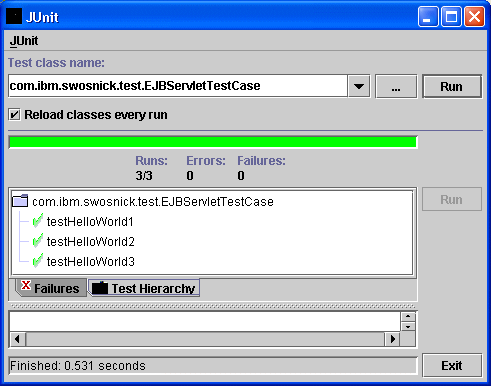
\includegraphics[width=\linewidth]{img/junit.png}
    \end{column}
  \end{columns}
\end{frame}
%%%%%%%%%%%%%%%%%%%%%%%%%%%%%%%%%%%%%%%%%%%%%%%%%%%%%%%%%%%%%%%%%%%%%%%%%%%%%%
\begin{frame}{Setting up test environment}
  \begin{block}{Purpose}
    \begin{itemize}
    \item Get things ready for testing.
    \item Create common instances, variables and data to use in tests.
    \end{itemize}
  \end{block}

  \begin{block}{Two kinds may co-exist}
    \begin{itemize}
    \item Setting up before each test function
      \begin{itemize}
      \item Named \framebox{\texttt{public void setUp()}} in JUnit 3.x
      \item Annotated \texttt{@Before} in JUnit 4.x
      \end{itemize}
    \item Setting up once for all 
      \begin{itemize}
      \item Placed in constructor in JUnit 3.x
      \item Annotated \texttt{@BeforeClass} in JUnit 4.x
      \end{itemize}
    \end{itemize}
  \end{block}
\end{frame}
%%%%%%%%%%%%%%%%%%%%%%%%%%%%%%%%%%%%%%%%%%%%%%%%%%%%%%%%%%%%%%%%%%%%%%%%%%%%%%
\begin{frame}{Cleaning test environment: Tearing down methods}
  \begin{block}{Purpose}
    \begin{itemize}
    \item Clean up after testing
    \item I.e., closing any files or connexions, etc
    \item Not used as often as setup methods
    \end{itemize}
  \end{block}
  \begin{block}{Two kinds may co-exist}
    \begin{itemize}
    \item Tearing down after each test function
      \begin{itemize}
      \item Named \framebox{\texttt{public void tearDown()}} in JUnit 3.x
      \item Annotated \texttt{@After} in JUnit 4.x
      \end{itemize}
    \item Tearing down once for all (JUnit 4.x only)
      \begin{itemize}
      \item Annotated \texttt{@AfterClass}
      \end{itemize}
    \end{itemize}
  \end{block}
\end{frame}
%%%%%%%%%%%%%%%%%%%%%%%%%%%%%%%%%%%%%%%%%%%%%%%%%%%%%%%%%%%%%%%%%%%%%%%%%%%%%%
\begin{frame}{Actually doing the tests}
  \begin{block}{Test functions}
    \begin{itemize}
    \item It is where the tests are performed
    \item Need one function per test case (which may call helper functions)

%    \medskip
    \item Name must start with \texttt{test} in JUnit 3.x
    \item Annotated \texttt{@Test} (in JUnit 4.x)
    \end{itemize}
  \end{block}\vspace{-.5\baselineskip}

  \begin{block}{Verifying results}
    \begin{itemize}
    \item All tests are verified with assertions.
    \item JUnit comes with an Assert class for this purpose
      \begin{itemize}
      \item public void assertTrue(String message, boolean condition)
      \item public void assertNotNull(String message, Object obj)
      \item public void assertEquals(String message, Object expected, Object actual)
      \item public void assertSame(String message, Object expected, Object
        actual)\\
        uses ==, not .equals()        
      \item public void assertFalse(String message, boolean condition)
      \item public void assertNotEquals(String message, Object expected, Object actual)
      \item public void assertNotSame(String message, Object expected, Object actual)
      \item public void fail(String message)
      \end{itemize}
    \end{itemize}
  \end{block}
\end{frame}
%%%%%%%%%%%%%%%%%%%%%%%%%%%%%%%%%%%%%%%%%%%%%%%%%%%%%%%%%%%%%%%%%%%%%%%%%%%%%%
\begin{frame}[fragile]{Example: Combination Lock (1/2)}
  \begin{block}{Data and setting up}
    \begin{Verbatim}
public class CombinationLockTest {
    // Locks with the specified combinations
    private CombinationLock lock00; // comb. 00
    private CombinationLock lock03; // comb. 03
    private CombinationLock lock12; // comb. 12
    private CombinationLock lock99; // comb. 99
    @Before
    public void setUp () {
        lock00 = new CombinationLock(0);
        lock03 = new CombinationLock(3);
        lock12 = new CombinationLock(12);
        lock99 = new CombinationLock(99);
    }
    ...
}      
    \end{Verbatim}
  \end{block}

  \begin{block}{Tear down not necessary here}
    \begin{itemize}
    \item object data will be deallocated automatically
    \item setup method overwrites instance variables
    \end{itemize}
  \end{block}
\end{frame}
%%%%%%%%%%%%%%%%%%%%%%%%%%%%%%%%%%%%%%%%%%%%%%%%%%%%%%%%%%%%%%%%%%%%%%%%%%%%%%
\begin{frame}[fragile]{Example: Combination Lock (2/2)}
  \begin{block}{Simple test method}
    \begin{Verbatim}
@Test
public void testOpenLock () {
    lock12.enter(3);
    lock12.enter(4);
    assertTrue(lock12.isOpen());
}      
    \end{Verbatim}
  \end{block}

  \begin{block}{Test method with helper}
    \begin{Verbatim}
@Test
public void testFirstDigitTwice () {
    closeLocks();
    firstDigitTwice(lock03,0,3);
    firstDigitTwice(lock12,1,2);
}
private void firstDigitTwice(CombinationLock lock, int first, int second) {
    lock.enter(first);
    lock.enter(first);
    assertFalse(lock.isOpen());
    lock.enter(second);
    assertTrue(lock.isOpen());
}
    \end{Verbatim}
  \end{block}
\end{frame}
%%%%%%%%%%%%%%%%%%%%%%%%%%%%%%%%%%%%%%%%%%%%%%%%%%%%%%%%%%%%%%%%%%%%%%%%%%%%%%%%%%
\begin{frame}{Going further with JUnit: TDD}
  \begin{block}{Test-Driven Development}
    \begin{itemize}
    \item That's a methodology to write code
    \item Aims at ease/productivity + code quality
    \end{itemize}
  \end{block}
  \begin{block}{Principle: \alert{Write the Test Cases First} (before the code)}
    \begin{itemize}
    \item Ensures that the codes actually get written
    \item Improves the interface: you're user of your own code before coding it
    \end{itemize}
  \end{block}
  \begin{block}{That's easy and pleasant to do}
    \begin{itemize}
    \item It's one of the ``agile development methodologies'', very
      light-weighted\\
      {\small More than just TDD in agile methods (but too long to say it all here)}
    \item Eclipse correction suggestion and ability to generate stubs very
      helpful 
    \item Try it for your next project
    \end{itemize}
  \end{block}
\end{frame}
%%%%%%%%%%%%%%%%%%%%%%%%%%%%%%%%%%%%%%%%%%%%%%%%%%%%%%%%%%%%%%%%%%%%%%%%%%%%%%%%%%%%%%%%%%%
\subsection{Right BICEP + CORRECT}
\begin{frame}{Right BICEPS}
  \begin{block}{Thinking of all mandatory test cases is difficult}
    \begin{itemize}
    \item I.e., challenging to discover all the ways a code might fail
    \item \structure{Good news:} Experience quickly gives a feel for what is likely to fail
    \end{itemize}
  \end{block}

  \begin{block}{Beginners need a bit of help  (until they get experienced)}
    \begin{itemize}
    \item Guidelines on what can fail
    \item Reminders of areas that are important to test
    \item These guidelines are not very complex, but quite useful/powerful
    \item See \structure{Software Systems and Architecture} [Scott Miller] for details
    \end{itemize}
  \end{block}
\end{frame}
%%%%%%%%%%%%%%%%%%%%%%%%%%%%%%%%%%%%%%%%%%%%%%%%%%%%%%%%%%%%%%%%%%%%%%%%%%
\begin{frame}{Right-BICEP}
  \begin{block}{Guidelines in a Nutshell}
    \begin{itemize}
    \item \structure{Right:} Are the results right?
    \item \structure{B:} Are all the \alert{b}oundary conditions CORRECT?
    \item \structure{I:} Can you check \alert{i}nverse relationships?
    \item \structure{C:} Can you \alert{c}ross-check results using other
      means?
    \item \structure{E:} Can you force \alert{e}rror conditions to happen?
    \item \structure{P:} Are \alert{p}erformance characteristics within bounds?
    \end{itemize}
  \end{block}
  
  \begin{block}{Right?}
    \begin{itemize}
    \item We need to compute what the correct result should be to test
    \item Quite often these can be inferred from the specification
    \item If the "right" results cannot be determined$\ldots$
      you shouldn't be writing code!
    \item If spec not completed [by client], assume what's correct, and
      fix afterward
    \end{itemize}
  \end{block}
\end{frame}
%%%%%%%%%%%%%%%%%%%%%%%%%%%%%%%%%%%%%%%%%%%%%%%%%%%%%%%%%%%%%%%%%%%%%%%%%%
\begin{frame}{B: Boundary Tests (1/3)} 

  \begin{block}{Discovering boundary conditions is crucial!}
    \begin{itemize}
    \item This is where most of the bugs generally live
    \item These are also the "edges" of our code 
    \end{itemize}
  \end{block}

  \begin{block}{Remember our little experience}
    \begin{itemize}
    \item We had to refine it several time our specifications
      \begin{itemize}
      \item Triangle with negative length
      \item Sort an empty array
      \end{itemize}
    \item The algorithm in exercise 3 of proof lab were false
      \begin{itemize}
      \item Failed to find smallest value if at the end of the array
      \end{itemize}
    \end{itemize}
  \end{block}
\end{frame}
%%%%%%%%%%%%%%%%%%%%%%%%%%%%%%%%%%%%%%%%%%%%%%%%%%%%%%%%%%%%%%%%%%%%%%%%%%%%%%%%%%%%%%%%%
\begin{frame}{B: Boundary Tests (2/3)}
  \begin{block}{Example of boundary conditions}
    \begin{itemize}
    \item \structure{Totally bogus, inconsistent input values}: filename of "\#()*\%)Q*\#\%\&@"
    \item \structure{Badly formatted data}: e-mail address without TLD (zastre@foo)
    \item \structure{Empty or missing values}: 0, 0.0, "", null
    \item \structure{Values above some reasonable expectation:} age of 10,000; \#children == 30
    \item \structure{Duplicates in lists meant to be free of duplicates}
    \item \structure{Ordered lists that are not ordered}\\
      {\small Also: Presorted lists passed to sort algorithms? reverse-sorted?}
    \item \structure{Things which arrive out of order? or out of expected order?}
    \end{itemize}
  \end{block}
\end{frame}
%%%%%%%%%%%%%%%%%%%%%%%%%%%%%%%%%%%%%%%%%%%%%%%%%%%%%%%%%%%%%%%%%%%%%%%%%%
\begin{frame}{B: Boundary Tests (3/3)}
  \begin{block}{Another guideline for boundaries: CORRECT}
    \begin{itemize}
    \item \structure{Conformance:} Does the value conform to an expected
      value?
    \item \structure{Ordering:} Is the set of values ordered or unordered as
      appropriate?
    \item \structure{Range:} Is the value within reasonable minimum and maximum
      values?
    \item \structure{Reference:} Does the code reference anything external that
      isn't under control? % of the code itself?
    \item \structure{Existence:} Does the value exist? (e.g., is non-null, non-
      zero, present in a set)
    \item \structure{Cardinality:} Are there exactly enough values?
    \item \structure{Time:} Is everything happening in order? At the right
      time? In time?
    \end{itemize}
  \end{block}
\end{frame}
%%%%%%%%%%%%%%%%%%%%%%%%%%%%%%%%%%%%%%%%%%%%%%%%%%%%%%%%%%%%%%%%%%%%%%%%%%
\begin{frame}{I: Check Inverse Relationships}
  \begin{block}{Some methods can be checked almost trivially}
    \begin{itemize}
    \item Data inserted in table should appear in a search immediately
      afterwards
    \item Lossless compression algorithm $\leadsto$ data uncompressed to the original value
    \item Check square-root calculation by squaring result (ensure it is "close
      enough")
    \end{itemize}
  \end{block}

  \begin{block}{Inverse Gotchas}
    \begin{itemize}
    \item You usually write the function/method and its inverse
    \item What if both are buggy? errors gets be masked
    \item Ideally, the inverse function is written by somebody else
      \begin{itemize}
      \item Square root example: use built-in multiplication
      \item Database insert: vendor-provided search routine to test insert
      \end{itemize}
    \end{itemize}
  \end{block}
\end{frame}
%%%%%%%%%%%%%%%%%%%%%%%%%%%%%%%%%%%%%%%%%%%%%%%%%%%%%%%%%%%%%%%%%%%%%%%%%%
\begin{frame}{C: Cross-check Using Other Means}
  \begin{block}{Idea 1: For methods without an inverse }
    \begin{itemize}
    \item Use a different algorithm to compute the result, and compare to yours
    \item For example, use a $O(n^2)$ sorting algorithm to check your
      $O(n\times log(n)$ one
    \end{itemize}
  \end{block}

  \begin{block}{Idea 2: Ensure that different pieces of the class's data ``add up''}
    \begin{itemize}
    \item Example: library system with book, copies
    \item "books out" + "books in library" should equal "total
      copies"
    \end{itemize}
  \end{block}
\end{frame}
%%%%%%%%%%%%%%%%%%%%%%%%%%%%%%%%%%%%%%%%%%%%%%%%%%%%%%%%%%%%%%%%%%%%%%%%%%
\begin{frame}{E: Force Error Conditions}
  \begin{block}{Production code defensive to system failures}
    \begin{itemize}
    \item \structure{Disks:} fill up
    \item \structure{Networks:} go down
    \item \structure{E-mail:} gets lost
    \item \structure{Programs:} crash
    \end{itemize}
  \end{block}
  \begin{block}{This also should to be tested}
    \begin{itemize}
    \item \structure{Easy:} invalid parameters
    \item \structure{Harder:} environmental errors
    \end{itemize}
  \end{block}
  \begin{block}{Environmental errors/constraints}
    \begin{itemize}
    \item Out of memory;  Out of disk space
%    \item Issues with wall-clock time
    \item Network availability and errors
    \item System load
    \item Limited colour palette; Very high or very low video resolution
    \item \ldots
    \end{itemize}
  \end{block}
\end{frame}
%%%%%%%%%%%%%%%%%%%%%%%%%%%%%%%%%%%%%%%%%%%%%%%%%%%%%%%%%%%%%%%%%%%%%%%%%%
\begin{frame}{P: Performance Characteristics}
  \begin{block}{What is the time performance as:}
    \begin{itemize}
    \item Input size grows?
    \item Problem sets become more complex
    \end{itemize}
  \end{block}

  \begin{block}{Idea: ``regression test'' on performance characteristics}
    \begin{itemize}
    \item Ensure that version N+1 is not awfully slower than version N
    \end{itemize}
  \end{block}

  \begin{block}{Very hard to ensure}
    \begin{itemize}
    \item Bad performance can come from external factors
    \item Performance not portable from machine to machine
    \item (even harder to ensure \textit{automatically})
    \end{itemize}
  \end{block}
\end{frame}
%%%%%%%%%%%%%%%%%%%%%%%%%%%%%%%%%%%%%%%%%%%%%%%%%%%%%%%%%%%%%%%%%%%%%%%%%%
\begin{frame}[fragile]{When to stop writing tests?}
  \begin{boitequote}{E. W. Dijkstra}
    Testing can only prove the presence of defects, not their absence.
  \end{boitequote}
  
  \begin{block}{Cynical answer (sad but true)}
    \begin{itemize}
    \item You're never done: each run of the system is a new test
      \begin{itemize}
      \item[$\Rightarrow$] Each bug-fix should be accompanied by a new
        regression test
      \end{itemize}       
    \item You're done when you are out of time/money
      \begin{itemize}
      \item Include test in project plan and \textbf{do not give in to pressure}
      \item ... in the long run, tests \textbf{save} time
      \end{itemize}
    \end{itemize}
  \end{block}

  \begin{block}{Statistical testing}
    \begin{itemize}
    \item Test until you've reduced failure rate under risk threshold
    \end{itemize}
    \centerline{\includegraphics{fig/test_statistical_testing.fig}}
  \end{block}
\end{frame}
%%%%%%%%%%%%%%%%%%%%%%%%%%%%%%%%%%%%%%%%%%%%%%%%%%%%%%%%%%%%%%%%%%%%%%%%%% 
\begin{frame}[fragile]{Why to test? (continued)}
  \concept{Because it helps ensuring that the system matches its specification}
  \bigskip

  \begin{block}{But not only (more good reason to test)}
    \begin{itemize}
    \item \structure{Traceability}
      \begin{itemize}
      \item Tests helps tracing back from components to the requirements that
        caused their presence
      \end{itemize}
    \item \structure{Maintainability}
      \begin{itemize}
      \item Regression tests verify that post-delivery changes do not break
        anything
      \end{itemize}
    \item \structure{Understandability}
      \begin{itemize}
      \item Newcomers to the system can read the test code to understand what
        it does
      \item Writing tests first encourage to make the interface really useable
      \end{itemize}
    \end{itemize}
  \end{block}
\end{frame}
%%%%%%%%%%%%%%%%%%%%%%%%%%%%%%%%%%%%%%%%%%%%%%%%%%%%%%%%%%%%%%%%%%%%%%%%%% 
%%%%%%%%%%%%%%%%%%%%%%%%%%%%%%%%%%%%%%%%%%%%%%%%%%%%%%%%%%%%%%%%%%%%%%%%%%%%%%%%%%
\section{Other Techniques for Practical Software Correctness}\sectionpage
%%%%%%%%%%%%%%%%%%%%%%%%%%%%%%%%%%%%%%%%%%%%%%%%%%%%%%%%%%%%%%%%%%%%%%%%%% 
\subsection{Design By Contract}
\begin{frame}{Introduction}
  \begin{block}{Design by Contract}
    \begin{itemize}
    \item Programming methodology trying to prevent code to diverge from specs
    \item Mistakes are possible
      \begin{itemize}
      \item while transforming requirements into a system
      \item while system is changed during maintenance
      \end{itemize}
    \end{itemize}
  \end{block}

  \begin{block}<2->{What's the difference with Testing?}
    \begin{itemize}
    \item Testing tries to diagnose (and cure) errors after the facts
    \item Design by Contract tries to prevent certain types of errors
    \end{itemize}
  \end{block}\vspace{-.5\baselineskip}

  \begin{block}<3->{Design by Contract is particularly useful in an Object-Oriented context}
    \begin{itemize}
    \item preventing errors in interfaces between classes\\
      {\small incl. subclass and superclass via subcontracting}
    \item preventing errors while reusing classes\\
      {\small incl. evolving systems, thus incremental and iterative
        development\\
        Example of the Ariane 5 crash} 
    \end{itemize}
  \end{block}

  \visible<4->{\concept{Use Design by Contract in combination with Testing!}}
\end{frame}
%%%%%%%%%%%%%%%%%%%%%%%%%%%%%%%%%%%%%%%%%%%%%%%%%%%%%%%%%%%%%%%%%%%%%%%%%% 
\begin{frame}{What is Design By Contract?}
  \begin{boitequote}{}
    View the relationship between two classes as a formal agreement, expressing
    each party's rights and obligations.~\hfill{\rm -- Bertrand Meyer}
  \end{boitequote}

  \begin{block}{Example: Airline Reservation}
    \begin{tabular}{p{.15\linewidth}|p{.37\linewidth}|p{.37\linewidth}}\hline
      &Obligations&Rights\\\hline
      Customer&
      \begin{itemize}\vspace{-.8\baselineskip}
      \item Be at Paris airport at least 3 hour before scheduled departure time
      \item Bring acceptable baggage
      \item Pay ticket price
      \end{itemize}\vspace{-1.2\baselineskip}
      &
      \begin{itemize}\vspace{-.8\baselineskip}
      \item Reach Los Angeles
      \end{itemize}
      \\\hline
      Airline&
      \begin{itemize}\vspace{-.8\baselineskip}
      \item Bring customer to Los Angeles
      \end{itemize}
      &
      \begin{itemize}\vspace{-.8\baselineskip}
      \item No need to carry passenger who is late
      \item has unacceptable baggage
      \item or has not paid ticket
      \end{itemize}\vspace{-1.2\baselineskip}
    \end{tabular}
  \end{block}
  \begin{itemize}
  \item Each party expects benefits (rights) and accepts obligations
  \item Usually, one party's benefits are the other party's obligations
  \item Contract is declarative: it is described so that both parties can
    understand \textit{what} service will be guaranteed without saying
    \textit{how}
  \end{itemize}
\end{frame}
%%%%%%%%%%%%%%%%%%%%%%%%%%%%%%%%%%%%%%%%%%%%%%%%%%%%%%%%%%%%%%%%%%%%%%%%%% 
\begin{frame}{Connecting back to Hoare logic}
  \begin{block}{Pre- and Post-conditions + Invariants}
    \begin{itemize}
    \item Obligations are expressed via pre- and post-conditions
      \begin{boitequote}{}
        If you promise to call me with the precondition satisfied, then I, in
        return promise to deliver a final state in which the postcondition is
        satisfied.
      \end{boitequote}
      \begin{center}
      pre-condition: {$x >= 9$} ~~~post-condition: {$x >= 13$}

      \framebox{component: {x := x + 5}}        
      \end{center}
      \vspace{-\baselineskip}
    \item and invariants
      \begin{boitequote}{}
        For all calls you make to me, I will make sure the invariant remains
        satisfied.
      \end{boitequote}
    \end{itemize}
  \end{block}

  \begin{block}{Isn't this pure documentation?}
    \begin{itemize}
    \item[(a)] Who will register these contracts for later reference (the notary)?\\
      \visible<2->{The source code}
    \item[(b)] Who will verify that the parties satisfy their contracts (the lawyers)?\\
      \visible<2->{The running system}
    \end{itemize}
  \end{block}
\end{frame}
%%%%%%%%%%%%%%%%%%%%%%%%%%%%%%%%%%%%%%%%%%%%%%%%%%%%%%%%%%%%%%%%%%%%%%%%%% 
\begin{frame}{Example: Stack}
  \begin{block}{Specification}
    \begin{itemize}
    \item \structure{Given}
      \begin{itemize}
      \item A stream of characters, length unknown
      \end{itemize}
    \item \structure{Requested}
      \begin{itemize}
      \item Produce a stream containing the same characters but in reverse
        order
      \item Specify the necessary intermediate abstract data structure
      \end{itemize}
    \end{itemize}
  \end{block}
  \bigskip
  \centerline{\includegraphics{fig/dbc_stack.fig}}
\end{frame}
%%%%%%%%%%%%%%%%%%%%%%%%%%%%%%%%%%%%%%%%%%%%%%%%%%%%%%%%%%%%%%%%%%%%%%%%%% 
\begin{frame}{Example: Stack Specification}
  \begin{tabbing}
    class stack\\
    ~~\=invariant: (isEmpty (this)) or (! isEmpty (this))\\
    \>\structure{/*} \=\structure{Implementors  promise that invariant holds
      after all methods return}\\
    \>\> \structure{(incl. constructors)*/}\\
    \>public char \alert{pop} ()\\
    \>\>require: !isEmpty(this)   ~~~~~~~~~~~~~~~~
                         \=\structure{/* Clients' promise (precondition) */}\\
    \>\>ensure: true     \>\structure{/* Implementors' promise
      (postcondition)}\\
    \>\>\>\structure{~~~~Here: nothing */}\\
    \>public void \alert{push}(char)\\
    \>\>require: true\\
    \>\>ensure: (!isEmpty(this))
       \>\structure{/* Implementors' promise: }\\
    \>\>~~~~~~~~~~~and (top(this)==char)
       \>\structure{~~~~Matches specification */}\\
    \>public void \alert{top} (char) : char\\
    \>\>require: \ldots \>\structure{/* left as an exercise */}\\
    \>\>ensure: \ldots\\
    \>public void \alert{isEmpty}() : boolean\\
    \>\>require: \ldots\\
    \>\>ensure: \ldots
  \end{tabbing}
\end{frame}
%%%%%%%%%%%%%%%%%%%%%%%%%%%%%%%%%%%%%%%%%%%%%%%%%%%%%%%%%%%%%%%%%%%%%%%%%% 
\begin{frame}[fragile]{Defensive Programming}
  \begin{block}{Redundant checks}
    \begin{itemize}
    \item Redundant checks are the naive way for including contracts in the
      source code
    \begin{columns}
      \begin{column}{.4\linewidth}
        \begin{Verbatim}
public char pop () {
  if (isEmpty (this)) {
    ... //Error-handling
  } else {
    ...}          
        \end{Verbatim}
      \end{column}
      \begin{column}{.6\linewidth}
        This is redundant code: it is the responsibility of the client to
        ensure the pre-condition!
      \end{column}
    \end{columns}
    \end{itemize}
  \end{block}

  \begin{block}{Redundant Checks Considered Harmful}
    \begin{itemize}
    \item Extra complexity\\
      {\small due to extra (possibly duplicated) code ... which must be
        verified as well}
    \item Performance penalty\\
      {\small Redundant checks cost extra execution time}
    \item Wrong context
      \begin{itemize}
      \item How severe is the fault? How to rectify the situation?
      \item A service provider cannot asses the situation, only the consumer
        can.
      \item Again: What happens if the precondition is not satisfied?
      \end{itemize}
    \end{itemize}
  \end{block}
\end{frame}
%%%%%%%%%%%%%%%%%%%%%%%%%%%%%%%%%%%%%%%%%%%%%%%%%%%%%%%%%%%%%%%%%%%%%%%%%% 
\begin{frame}{Assertions}
  \concept{Any boolean expression we expect to be true at some point}

  \begin{block}{Advantages}
    \begin{itemize}
    \item Help in writing correct software 
      {\small(formalizing invariants, and pre/post-conditions)}
    \item Aid in maintenance of documentation
      {\small(specifying contracts \alert{in the source code})}\\
      $\Rightarrow$ tools to extract interfaces and contracts from source code
    \item Serve as test coverage criterion 
      {\small (Generate test cases that falsify assertions)}
    \item Should be configured at compile-time 
      {\small (to avoid performance penalties in prod)}
    \end{itemize}    
  \end{block}

  \begin{block}{What happens if the precondition is not satisfied?}
    \begin{itemize}
    \item When an assertion does not hold, throw an exception
    \end{itemize}
  \end{block}
\end{frame}
%%%%%%%%%%%%%%%%%%%%%%%%%%%%%%%%%%%%%%%%%%%%%%%%%%%%%%%%%%%%%%%%%%%%%%%%%% 
\begin{frame}{Assertions in Programming Languages}
  \begin{block}{Eiffel}
    \begin{itemize}
    \item Eiffel is designed as such ... but only used for correction (not documentation)
    \end{itemize}
  \end{block}

  \begin{block}{C++}
    \begin{itemize}
    \item assert.h does not throw an exception, but close program
    \item Possible to mimick. Documentation extraction rather difficult
    \end{itemize}
  \end{block}

  \begin{block}{Smalltalk}
    \begin{itemize}
    \item Easy to mimic, but compilation option requires some language idioms
    \item Documentation extraction is possible (style JavaDoc)
    \end{itemize}
  \end{block}

  \begin{block}{Java}
    \begin{itemize}
    \item Assert is standard since Java 1.4 ... very limited
    \item JML provide a mechanism ... but not ported to Java 5 (damn
      genericity)
    \item Modern Jass seems very promising, but needs more polishing
    \end{itemize}
  \end{block}
\end{frame}
%%%%%%%%%%%%%%%%%%%%%%%%%%%%%%%%%%%%%%%%%%%%%%%%%%%%%%%%%%%%%%%%%%%%%%%%%% 
%\subsection{Design by Contract vs. Testing}
\begin{frame}{Design by Contract vs. Testing}
  \begin{block}{They serve the same purpose}
    \begin{itemize}
    \item Design by contract \textit{prevents} errors; Testing \textit{detect}
      errors
    \item[$\leadsto$] One of them should be sufficient!
    \end{itemize}
  \end{block}

  \begin{block}{They are complementary}\medskip
    None of the two guarantee correctness ... but the sum is more than the
    parts
    \begin{itemize}
    \item Testing detects wide range of coding mistakes\\
      ... design by contract prevents specific mistakes due to incorrect
      assumption
    \item Design by contract ease black box testing by formalizing
      spec 
    \item Condition testing verify whether all assertions are satisfied\\
      {\small(whether parties satisfy their obligations)}
    \end{itemize}
  \end{block}
\end{frame}
%%%%%%%%%%%%%%%%%%%%%%%%%%%%%%%%%%%%%%%%%%%%%%%%%%%%%%%%%%%%%%%%%%%%%%%%%%%%%%%%%%
\subsection{Fuzzing}\subsectionpage
\begin{frame}[squeeze]{Fuzzing big picture}
  \begin{enumerate}
  \item Intercept the data an application gets from its environment
  \item \alert{Fuzz it}, i.e. provide data vaguely resembling to expected
    one\\ 
    {\small (sort of model-checking, exploring only execution paths close to
      the usual one)}
  \end{enumerate}

  \centerline{\includegraphics[scale=.8]{fig/test_fuzzing.fig}}

  \begin{block}{Why? Motivation}\vspace{-.2\baselineskip}
    \begin{itemize}
    \item It's a security assessment method:\\
      {\small if you can get the application to segfault, it must be a buffer overflow
      to exploit}
    \item Easy to write some tests w/o system knowledge\\
      {\small $\Rightarrow$ launch a fuzzer when arriving in company, it may
        find something interesting}
    \item One of the best price/quality ratio
    \end{itemize}
  \end{block}\vspace{-.4\baselineskip}

  \begin{block}{Target applications}\vspace{-.2\baselineskip}
    \begin{itemize}
    \item Classically, network protocols; Recently used on media files
    \end{itemize}
  \end{block}
\end{frame}
%%%%%%%%%%%%%%%%%%%%%%%%%%%%%%%%%%%%%%%%%%%%%%%%%%%%%%%%%%%%%%%%%%%%%%%%%%%%
\begin{frame}{How to actually fuzz the data?}
  \begin{block}{Brute force: \alert{random}}
    \begin{itemize}
    \item Pick a byte in the stream, and change its value
    \item[\Smiley] Really easy to do
    \item[\Frownie] Get easily caught by checksums
    \item[\Frownie] ``Interesting changes'' are rather improbable
    \end{itemize}
  \end{block}

  \begin{block}{Refined manner: \alert{templating}}
    \begin{itemize}
    \item Understand the logic of the stream
    \item[\Smiley] Pass checksums and easy validity protection levels
    \item[\Frownie] Rather hard to do
    \item[\Frownie] Fuzzing process becomes stream-dependent\\
      {\small no longer first tool to use: you need to understand stream first}
    \end{itemize}
  \end{block}

  \begin{block}{Some research leads}
    \begin{itemize}
    \item \structure{Stateful fuzzing:} Build a protocol automaton, test
      invalid transitions
    \item \structure{Automatic~templating:}~Extend~\texttt{file}~format~%
      metagrammar,use~almost~valid~data
    \end{itemize}
  \end{block}
\end{frame}
%%%%%%%%%%%%%%%%%%%%%%%%%%%%%%%%%%%%%%%%%%%%%%%%%%%%%%%%%%%%%%%%%%%%%%%%%%%%%
\subsection{Formal Methods}\subsectionpage
\begin{frame}{Formal Methods}
  \alert{\large Goal:} Develop safe software using automated methods
  \begin{itemize}
  \item Strong mathematical background
  \item<2-> Safe $\equiv$ respect some given properties
  \end{itemize}

  \begin{block}<2->{Kind of properties shown}
    \begin{itemize}
    \item \structure{Safety:} the car does not start without the key
    \item \structure{Liveness:} if I push the break paddle, the car will
      eventually stop
    \end{itemize}
  \end{block}
\end{frame}
%%%%%%%%%%%%%%%%%%%%%%%%%%%%%%%%%%%%%%%%%%%%%%%%%%%%%%%%%%%%%%%%%%%%%%%%%%%%%%%%%%
\begin{frame}[squeeze]{Existing Formal Methods}
  \centerline{\includegraphics[scale=.7]{fig/test_formal_methods.fig}}

  \begin{block}{Proof of programs}
    \begin{itemize}
    \item In theory, applicable to any class of program
    \item In practice, quite tedious to use\\
      often limited to help a specialist doing the actual work {\small(system state explosion)}
    \end{itemize}
  \end{block}\vspace{-.3\baselineskip}

   \begin{block}{Model-checking}
     \begin{itemize}
     \item \structure{Goal:} Shows that a system:
       \begin{itemize}
       \item[(safety)] never evolves to a faulty state from a given initial state
       \item[(liveness)] always evolve to the wanted state {\small(stopping)} from a
         given state {\small(breaking)}
       \end{itemize}
     \item[\Frownie] Less generic than proof: lack of faulty states \alert{for all}
       initial state?
     \item[\Smiley] Usable by non-specialists (at least, by \textit{less-specialists})
     \end{itemize}
   \end{block} \vspace{-.3\baselineskip}

   \begin{block}{Static Checking}
     \begin{itemize}\vspace{-.2\baselineskip}
     \item Automatic analyse of the source code {\small(data flow analysis; theorem proving)}
     \item Completely automated, you should use these tools, even if partial coverage
     \end{itemize}
   \end{block}
\end{frame}
%%%%%%%%%%%%%%%%%%%%%%%%%%%%%%%%%%%%%%%%%%%%%%%%%%%%%%%%%%%%%%%%%%%%%%%%%%
\begin{frame}[squeeze]{Example of problem to detect: Race Condition}
  $x$ is a shared variable; $Alice$ adds 2, $Bob$ adds 5;
  \alert{Correct result : $x=7$}
  \begin{enumerate}
  \item[a.] Read the value of shared variable $x$ and store it locally
  \item[b.] Modify the local value (add 5 or 2)
  \item[c.] Propagate the local variable into the shared one
  \end{enumerate}

  \visible<2->{
    \begin{itemize}
    \item \structure{Execution of $Alice$ \textbf{then} $Bob$ or opposite:} \alert{result = 7}
    \item \structure{Interleaved execution:} \alert{result = 2 or 5} (depending
      on last propagator)
    \end{itemize}
  }


  \visible<3->{
    \alert{\textbf{Model-checking}: traverse graph of executions checking for
      properties}\vspace{-\baselineskip}

    \centerline{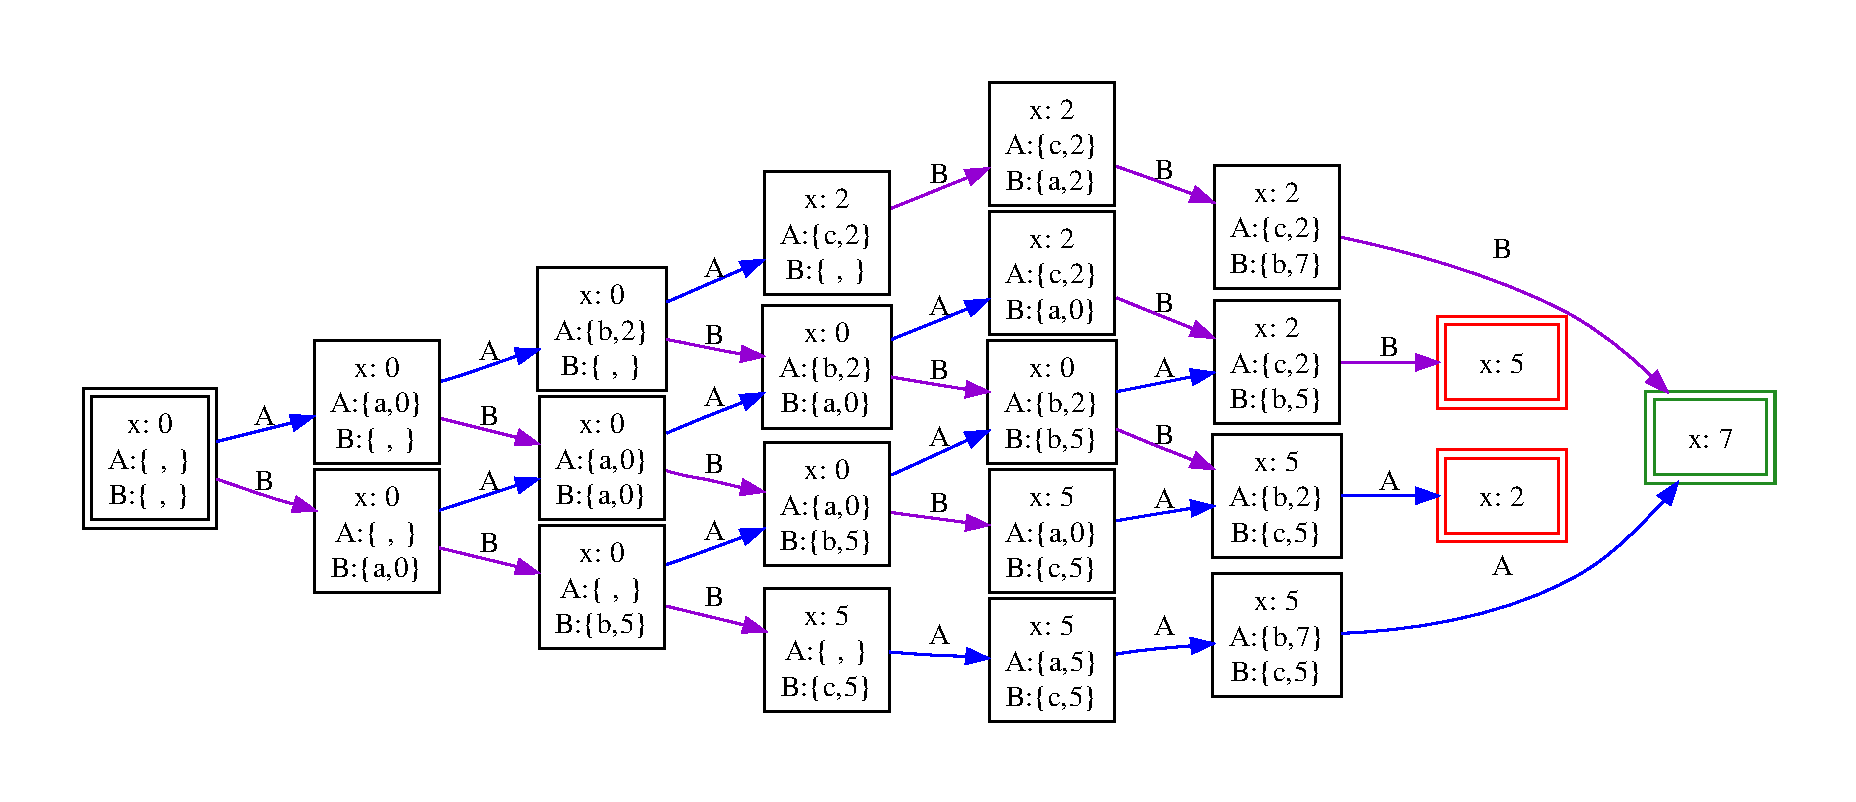
\includegraphics[height=12\baselineskip]{fig/test_mutex.pdf}}
    \vspace{-1.5\baselineskip}
  }%
  \visible<4->{%
    \begin{columns}
      \begin{column}{.5\linewidth}
        \begin{itemize}
        \item Safety: assertions on each node
        \end{itemize}
      \end{column}
      \begin{column}{.5\linewidth}
        \begin{itemize}
        \item Liveness by studying graph (cycle?)
        \end{itemize}
      \end{column}
    \end{columns}
  }
\end{frame}
%%%%%%%%%%%%%%%%%%%%%%%%%%%%%%%%%%%%%%%%%%%%%%%%%%%%%%%%%%%%%%%%%%%%%%%%%%%%%%%%%% 

\begin{frame}{Model-Checking Big Picture}
  \begin{enumerate}
  \item User writes \alert{Model} {\small(formal writing of algorithm)} and
    \alert{Specification} {\small(set of properties)}
  \item Each decision point in model (if, input data) $\leadsto$ a branch
    in model state space
  \item Check safety properties on each encountered node (state)
  \item Store encountered nodes (to avoid looping) and transitions (to check liveness)
  \item Process until:
    \begin{itemize}
    \item State space completely traversed ($\Rightarrow$ model verified
      against this specification)
    \item One of the property does not hold (the path until here is a
      counter-example)
    \item We run out of resource ("state space explosion")
    \end{itemize}
  \end{enumerate}

  \centerline{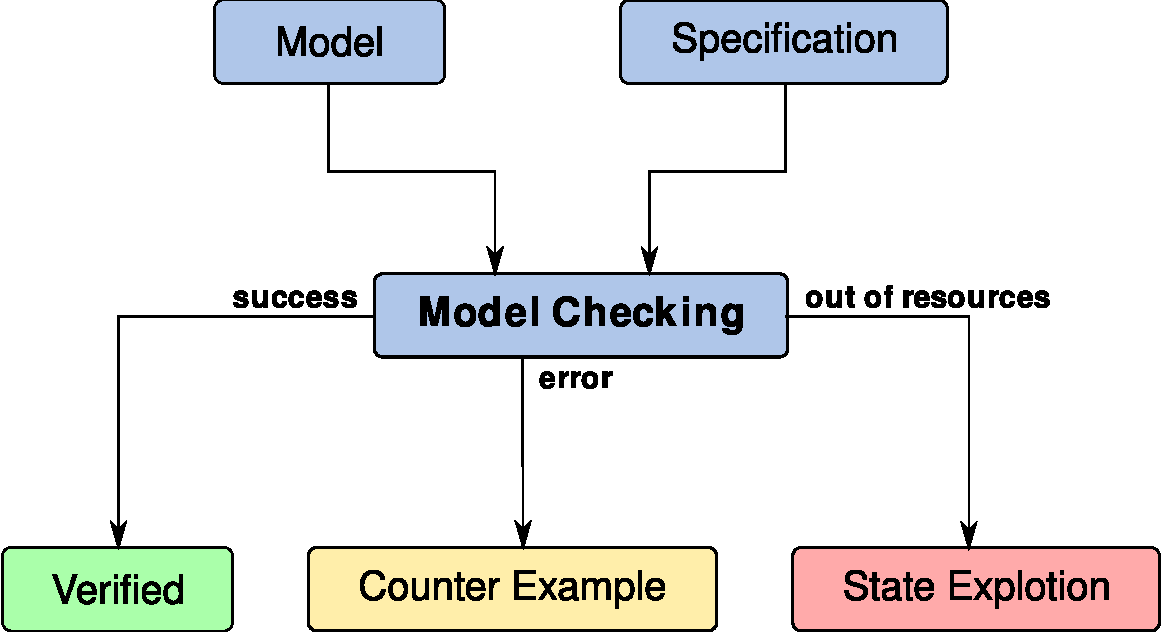
\includegraphics[width=.56\linewidth]{fig/test_modelchecking.pdf}}
\end{frame}
%%%%%%%%%%%%%%%%%%%%%%%%%%%%%%%%%%%%%%%%%%%%%%%%%%%%%%%%%%%%%%%%%%%%%%%%%%%%%%%%
\section{Conclusion}\mypartpage
%%%%%%%%%%%%%%%%%%%%%%%%%%%%%%%%%%%%%%%%%%%%%%%%%%%%%%%%%%%%%%%%%%%%%%%%%%%%%%%%%%%%%%%
\begin{frame}[t,fragile,squeeze]{A Comparison of Bug Finding Tools for Java}
  \vspace{-1.2\baselineskip}~\hfill{\footnotesize Rutar, Almazan, Foster,
    U. Maryland -- ISSRE04}
  \medskip
  \begin{columns}
    \begin{column}{.41\linewidth}
      \begin{Verbatim}[frame=single,label=Example code,fontsize=\footnotesize,numbers=left,numbersep=1pt]
import java.io.*;
public class Foo{
 private byte[] b;
 private int length;
 Foo(){ length = 40;
  b = new byte[length]; }
 public void bar(){
  int y;
  try {
   FileInputStream x =
    new FileInputStream("z");
   x.read(b,0,length);
   x.close();}
  catch(Exception e){
   System.out.println("Oopsie");}
  for(int i=1; i<=length; i++){
   if (Integer.toString(50) ==
             Byte.toString(b[i]))
   System.out.print(b[i] + " ");
  }
 }
}
      \end{Verbatim}
    \end{column}
    \begin{column}{.55\linewidth}
      \begin{block}{Defects of this code}
        \visible<2->{
          \begin{itemize}
          \item[l8] W: Unused variable
          \item[l12] W: Return of read() ignored
          \item[l14] W: Stream may not be closed
          \item[l17] \alert{E:} == to compare strings
          \item[l18] \alert{E:} may acces out of bound
          \item[l18] FP: possible null-dereference to b
          \end{itemize}
        }        
      \end{block}\vspace{-.6\baselineskip}

      \begin{block}<3->{Some tools for Java}\medskip
        \resizebox{\linewidth}{!}{
          \begin{tabular}{|c|c|c|c|}\hline
            Name&Input&Interface&Technology\\\hline
            Bandera&Source&CL, GUI&Model checking\\\hline
            ESC/Java&Source+spec&CL, GUI&Theorem proving\\\hline
            FindBugs&Bytecode&CL,GUI,Ant,IDE&Syntax, data-flow\\\hline
            JLint&Bytecode&CL&Syntax, data-flow\\\hline
            PMD&Source&CL,GUI,Ant,IDE&Syntax\\\hline
          \end{tabular}
        }
      \end{block}\vspace{-.2\baselineskip}

      \begin{block}<4->{No tool is perfect/sufficient}
        \begin{itemize}\vspace{-.4\baselineskip}
        \item All detect something
        \item Some give false positive {\small(b inited in ctor)}
        \item All have false negative
        \end{itemize}
      \end{block}
    \end{column}
  \end{columns}
\end{frame}
%%%%%%%%%%%%%%%%%%%%%%%%%%%%%%%%%%%%%%%%%%%%%%%%%%%%%%%%%%%%%%%%%%%%%%%%%
\begin{frame}{Conclusion}
  \begin{block}{Failure is not an option.
It comes bundled with software.}
    \begin{itemize}
    \item \structure{Testing} searches for defects\\
      {\small But not that easy and endless?}
    \item \structure{Proof} tries to ensure that there is no defect\\
      {\small But quite heavy-weighted}
    \item \structure{Automatic tools} (static checking, theorem provers) may help\\
      {\small But none is enough/sufficient (false negatives); all have false positives}
    \item \structure{Design by Contract} constitutes a global (methodological) answer\\
      {\small Too bad that nobody use it / that Java offers no tool support for
        it (yet?)}
    \end{itemize}
  \end{block}

  \begin{block}{Optimistic Last Note}
    \begin{itemize}
    \item That's a hot research topic, things move fast
    \item Tools improve quickly, you really should learn to use them
    \item Methodologies exist {\small(DBC, TDD)}, you should try to follow them
    \end{itemize}
  \end{block}
\end{frame}
%%%%%%%%%%%%%%%%%%%%%%%%%%%%%%%%%%%%%%%%%%%%%%%%%%%%%%%%%%%%%%%%%%%%%%%%%%%%
\begin{frame}{Bibliography for this chapter (and previous one)}
  \begin{block}{Lectures}
    \begin{itemize}
    \item \structure{Testing, Debugging, and Verification} (W. Ahrendt,
      R. H\"ahnle -- U. G\"oteborgs)
      \url{www.cse.chalmers.se/edu/year/2009/course/TDA566}
    \item \structure{Software Engineering} (Serge Demeyer -- U. Antwerpen)
      \url{http://www.lore.ua.ac.be/Teaching/SE3BAC/}
    \item \structure{Software Systems and Architecture} (Scott Miller -- U. of
      Victoria)\\
      \url{http://samiller.ece.uvic.ca/courses/SENG271/2009/05/}
    \item \structure{JUnit} (Dirk Hasselbalch -- U. Copenhagen) 
      \url{http://isis.ku.dk/kurser/blob.aspx?feltid=217458}
    \end{itemize}    
  \end{block}
  \begin{block}{Other}
    \begin{itemize}
    \item \structure{Test Infected: Programmers Love Writing Tests} (Tutorial on JUnit)
      \url{http://www.cril.univ-artois.fr/~leberre/MI32001/TESTING/junit3.7/doc/testinfected/ntesting_fr.htm}
    \end{itemize}    
  \end{block}
\end{frame}
% LocalWords:  LocalWords
%% coding: utf-8
